\documentclass[runningheads]{llncs}
%
\usepackage[T1]{fontenc}
\usepackage{tikz}
\usetikzlibrary{arrows.meta, positioning, calc, backgrounds, fit, shadows.blur}
\usetikzlibrary{shadows}
% T1 fonts will be used to generate the final print and online PDFs,
% so please use T1 fonts in your manuscript whenever possible.
% Other font encodings may result in incorrect characters.
%
% Hyperref package for clickable links
\usepackage{hyperref}
%
\usepackage{graphicx}
% Used for displaying a sample figure. If possible, figure files should
% be included in EPS format.
%
% If you use the hyperref package, please uncomment the following two lines
% to display URLs in blue roman font according to Springer's eBook style:
\usepackage{color}
\renewcommand\UrlFont{\color{blue}\rmfamily}
\urlstyle{rm}
\usepackage{amsmath}
\usepackage{amssymb}
\usepackage{tikz}
\usetikzlibrary{positioning,arrows.meta,fit,backgrounds}
%\usepackage{algorithm}
%\usepackage{algpseudocode}
\usepackage[ruled,vlined]{algorithm2e}
\usepackage{fixme}
\fxsetup{draft}


\allowdisplaybreaks

\newcommand{\rGB}{\textsc{$r$-GB} }
\newcommand{\rGBP}{$r$-GBP }

\makeatletter
\AtBeginDocument{%
	\renewcommand\doi[1]{}%
}
\makeatother

% cSpell:enable

\begin{document}
	
 
\subsection{Xzyme workflow visualization}
  
\begin{figure}[!ht]
	\raggedright
	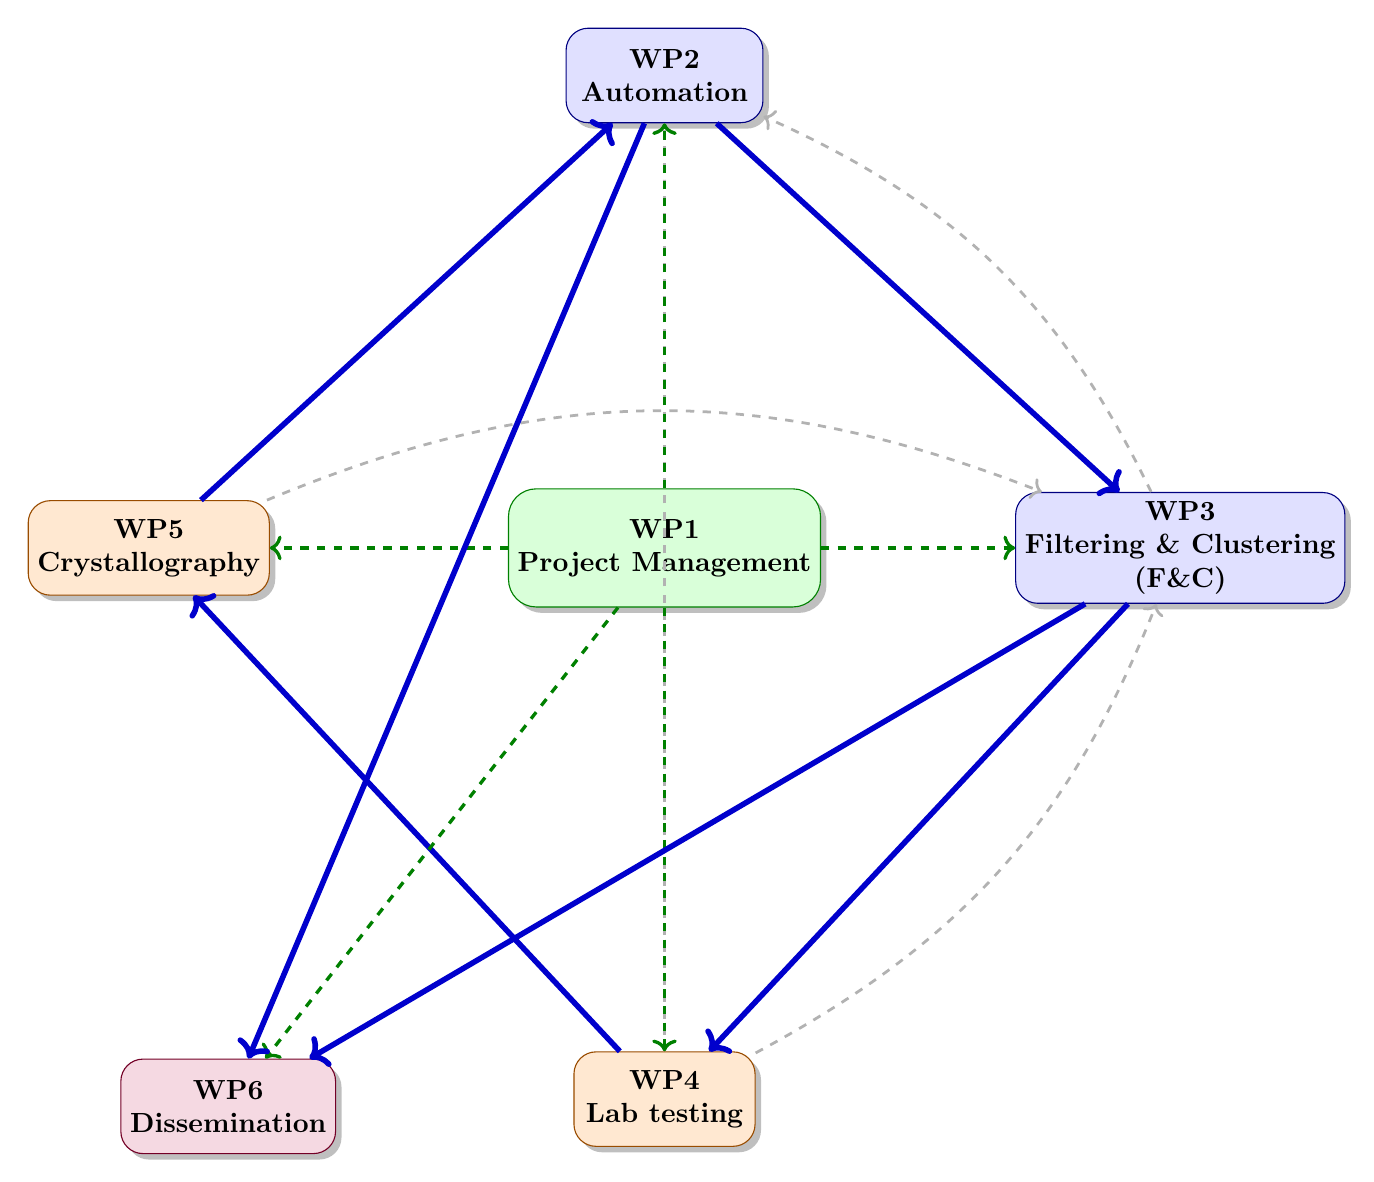
\begin{tikzpicture}[xshift=-2.5cm, 
		every node/.style={draw, rectangle, rounded corners, minimum width=1.0cm, minimum height=0.3cm, align=center},
		mainarrow/.style={->, line width=2pt, color=blue!80!black},
		feedback/.style={->, dashed, line width=1pt, color=gray!60},
		mgmt/.style={->, dashed, line width=1.2pt, color=green!50!black},
		lab/.style={
			draw,
			dashed,
			rounded corners=6pt,
			fill=gray!8,
			font=\small,
			align=center,
			inner sep=4pt
		},
		wp/.style={
			draw,
			rectangle,
			rounded corners=8pt,
			minimum width=2.5cm,
			minimum height=1.2cm,
			align=center,
			font=\bfseries,
			fill=blue!12,
			draw=blue!50!black,
			drop shadow
		},
		wp_exp/.style={
			draw,
			rectangle,
			rounded corners=8pt,
			minimum width=2.3cm,
			minimum height=1.2cm,
			align=center,
			font=\bfseries,
			fill=orange!18,
			draw=orange!60!black,
			drop shadow
		},
		wp_mgmt/.style={
			draw,
			rectangle,
			rounded corners=10pt,
			minimum width=3cm,
			minimum height=1.5cm,
			align=center,
			font=\bfseries,
			fill=green!15,
			draw=green!50!black,
			drop shadow
		},
		wp_diss/.style={
			draw,
			rectangle,
			rounded corners=8pt,
			minimum width=2.5cm,
			minimum height=1.2cm,
			align=center,
			font=\bfseries,
			fill=purple!15,
			draw=purple!60!black,
			drop shadow
		}
		]
		
		% --- Core circular WPs ---
		\node[wp] (WP2) at (90:6cm) {WP2\\Automation};
		\node[wp] (WP3) at (0:6.55cm) {WP3\\Filtering \& Clustering \\ (F\&C)};
		\node[wp_exp] (WP4) at (-90:7cm) {WP4 \\ Lab testing};
		\node[wp_exp] (WP5) at (180:6.55cm) {WP5\\Crystallography};
		
		% --- NEW: Center WP1 ---
		\node[wp_mgmt] (WP1) at (0,0) {WP1\\Project Management};
		
		% --- NEW: WP6 on the left ---
		\node[wp_diss] (WP6) at (-128:9cm) {WP6\\Dissemination};
		
		% --- Primary workflow ---
		\draw[mainarrow] (WP2) to node[midway, above, draw=none]{} (WP3);
		\draw[mainarrow] (WP3) to node[midway, above, draw=none]{} (WP4);
		\draw[mainarrow] (WP4) to node[midway, above, draw=none]{} (WP5);
		\draw[mainarrow] (WP5) to node[midway, above, draw=none]{} (WP2);
		
		% --- Feedback loops ---
		\draw[feedback] (WP3) to[bend right=20] node[midway, above, draw=none]{} (WP2);
		\draw[feedback] (WP4) to[bend right=20] node[midway, above, draw=none]{} (WP3);
		\draw[feedback] (WP4) to[bend right=0] node[midway, above, draw=none]{} (WP2);
		\draw[feedback] (WP5) to[bend right=-22] node[midway, above, draw=none]{} (WP3);
		
		% --- NEW: Management connections (WP1 to all) ---
		\draw[mgmt] (WP1) -- (WP2);
		\draw[mgmt] (WP1) -- (WP3);
		\draw[mgmt] (WP1) -- (WP4);
		\draw[mgmt] (WP1) -- (WP5);
		\draw[mgmt] (WP1) -- (WP6);
		
		% --- NEW: WP6 connections ---
		\draw[mainarrow] (WP2) to[bend left=0] (WP6);
		\draw[mainarrow] (WP3) to[bend left=0] (WP6);
		
		% --- Legends ---
		%\node[lab, align=left] at (-3.8, -9.0)
		%{ \textbf{Primary Workflow Loop} \\
		%	I. Enzyme Mimic Generation \\
		%	II. Reliable Enzyme Mimic Design \\
		%	III. Crystallographic Validation \\
		%	IV. Structure-Guided Workflow Adaptation
		%};
		
		%\node[lab, align=left] at (5.0, -9.0)
		%{ \textbf{Feedback and Refinement Loops} \\
		%	A. Workflow adjustment \\
		%	B. Filtering \& Clustering refinement \\
		%	C. Lab-driven workflow adaptation \\
		%	D. Structure-guided refinement };
		
	\end{tikzpicture}
\end{figure}
 

 
 \end{document}
